\documentclass[conference]{IEEEtran}
\IEEEoverridecommandlockouts
% Paquetes
\usepackage{cite}
\usepackage{amsmath,amssymb,amsfonts}
\usepackage{algorithmic}
\usepackage{graphicx}
\usepackage{textcomp}
\usepackage{xcolor}
\usepackage{url}
\usepackage{booktabs}
\usepackage{subcaption}
\usepackage[spanish]{babel}

\def\BibTeX{{\rm B\kern-.05em{\sc i\kern-.025em b}\kern-.08em
    T\kern-.1667em\lower.7ex\hbox{E}\kern-.125emX}}

\begin{document}

\title{SmartChimera: Graph-Based Software Team Assembly with Hybrid Risk Analysis for Bus Factor Mitigation}

\author{
\IEEEauthorblockN{Santiago Enrique Palma Apaza}
\IEEEauthorblockA{\textit{Escuela Profesional de Ingeniería de Sistemas} \\
\textit{Universidad Nacional de San Agustín}\\
Arequipa, Perú \\
spalma@unsa.edu.pe}
\and
\IEEEauthorblockN{Germán Arturo Chipana Jerónimo}
\IEEEauthorblockA{\textit{Escuela Profesional de Ingeniería de Sistemas} \\
\textit{Universidad Nacional de San Agustín}\\
Arequipa, Perú \\
gchipanaj@unsa.edu.pe}
\and
\IEEEauthorblockN{Leonardo Juan José Baca Calsin}
\IEEEauthorblockA{\textit{Escuela Profesional de Ingeniería de Sistemas} \\
\textit{Universidad Nacional de San Agustín}\\
Arequipa, Perú \\
lbacac@unsa.edu.pe}
}

\maketitle

\begin{abstract}
El Bus Factor representa el número mínimo de desarrolladores cuya salida simultánea colapsaría un proyecto de software, constituyendo un riesgo crítico para la continuidad organizacional. Este artículo presenta SmartChimera, un sistema basado en grafos que mitiga este riesgo sin depender de modelos de IA tipo caja negra. A diferencia de enfoques que requieren datos históricos extensivos, SmartChimera implementa una arquitectura determinística basada en dos motores principales: (1) Un detector híbrido de linchpins que combina Centralidad de Intermediación (algoritmo de Brandes) con métricas de dependencia de proyectos, y (2) Un algoritmo de ensamblaje de equipos de modo dual guiado por perfiles de misión (Resiliente vs. Rendimiento). Validamos el sistema mediante experimentos estadísticos rigurosos (N=500 pruebas), demostrando mejoras significativas sobre métodos base (p < 0.001, d de Cohen = 4.73). Los resultados muestran que SmartChimera logra puntuaciones de Bus Factor 33\% más altas y 100\% de cobertura de habilidades comparado con baselines greedy, Hungarian y aleatorios.
\end{abstract}

\begin{IEEEkeywords}
Bus Factor, Formación de Equipos, Teoría de Grafos, Gestión de Riesgos, Ingeniería de Software, Centralidad de Intermediación, Beam Search
\end{IEEEkeywords}

\section{Introducción}

El desarrollo de software moderno enfrenta una vulnerabilidad crítica: la dependencia excesiva en desarrolladores clave. El \textit{Bus Factor} (BF), introducido por Avelino et al. \cite{avelino2016novel}, cuantifica el riesgo de concentración de conocimiento. Estudios empíricos revelan que el 50\% de proyectos de código abierto tienen BF$\leq$2 \cite{avelino2016novel}, exponiendo fragilidad sistémica.

La rotación de desarrolladores amplifica este riesgo. Foucault et al. \cite{foucault2015impact} demuestran que las salidas de desarrolladores principales incrementan defectos en 40-60\%. Lin et al. \cite{lin2017developer} reportan que la pérdida de conocimiento tácito \cite{ryan2013acquiring} genera disrupciones arquitectónicas severas \cite{maccormack2012exploring}. La coordinación de expertos en redes sociales \cite{meneely2008predicting} y la propiedad colectiva del código \cite{maruping2009role} actúan como factores mitigantes frecuentemente ignorados.

Las soluciones actuales emplean optimización NP-hard \cite{lappas2009finding} o modelos de machine learning que requieren datasets masivos e inmaculados—poco realistas para la mayoría de empresas \cite{saeedi2025survey, ma2020data}. SmartChimera aborda esta brecha mediante \textbf{heurísticas determinísticas} y grafos de colaboración explícitos \cite{caglayan2013emergence}, eliminando el entrenamiento de modelos mientras asegura auditabilidad total.

\subsection{Contribuciones}

Este trabajo presenta tres contribuciones novedosas:

\begin{enumerate}
    \item \textbf{Métrica de Riesgo Híbrida:} Un algoritmo de detección de linchpins que combina Centralidad de Intermediación (topología de red) con Peso de Proyecto (distribución de carga) usando ponderación equitativa optimizada empíricamente ($\alpha=\beta=0.5$).
    
    \item \textbf{Estrategia de Ensamblaje de Modo Dual:} Marco de perfiles de misión que habilita formación de equipos consciente del contexto—modo Resiliente (minimizar riesgo) vs. modo Rendimiento (maximizar experiencia).
    
    \item \textbf{Validación Rigurosa:} Comparación estadística (N=500 pruebas) contra baselines greedy, Hungarian y aleatorio, demostrando mejoras significativas (p < 0.001) en Bus Factor, cobertura de habilidades y métricas de riesgo.
\end{enumerate}

\section{Trabajo Relacionado}

\subsection{Bus Factor y Detección de Linchpins}

Avelino et al. \cite{avelino2016novel} pioneros en la medición de Bus Factor usando análisis de control de versiones, identificando el conjunto mínimo de desarrolladores cuya remoción detiene el desarrollo. Su trabajo se enfoca en \textit{detección} pero no mitigación. Nuestra métrica híbrida extiende esto combinando centralidad de red social con dependencia de proyectos, capturando tanto cuellos de botella de comunicación como concentración de carga de trabajo.

Joblin et al. \cite{joblin2017evolutionary} modelan redes de commits como grafos de colaboración, habilitando análisis basado en centralidad. Adoptamos este fundamento de teoría de grafos pero lo mejoramos con estrategias de ponderación específicas a misiones.

\subsection{Algoritmos de Formación de Equipos}

Lappas et al. \cite{lappas2009finding} formalizan la formación de equipos como un problema NP-hard, proponiendo soluciones exactas vía satisfacción de restricciones. Aunque algorítmicamente óptimo, su enfoque requiere búsqueda exhaustiva inadecuada para recomendaciones en tiempo real. SmartChimera emplea beam search—una expansión greedy de ancho controlado que provee soluciones casi-óptimas con complejidad polinomial.

Falkner et al. \cite{falkner2016scalable} exploran tecnologías de restricciones para composición de equipos. Nuestros perfiles de misión pueden verse como restricciones suaves, permitiendo ajuste guiado por políticas sin alterar algoritmos centrales.

Dave y Varshney \cite{dave2018combined} combinan emparejamiento de habilidades con compatibilidad social. SmartChimera extiende esto incorporando Bus Factor como criterio de optimización explícito mediante el término de penalización BC.

\subsection{Posicionamiento}

A diferencia de trabajos previos, SmartChimera es:
\begin{itemize}
    \item \textbf{Determinístico:} Sin modelos caja negra que requieren datos de entrenamiento
    \item \textbf{Adaptativo:} Estrategia de modo dual se ajusta a diferentes fases del proyecto
    \item \textbf{Transparente:} Justificación basada en grafos visible para gerentes
    \item \textbf{Validado:} Comparación estadística rigurosa contra baselines
\end{itemize}

\section{Metodología}

\subsection{Modelo de Grafo}

Modelamos la organización como un grafo de colaboración ponderado $G = (V, E)$, donde $V$ representa empleados y $E$ denota relaciones de colaboración \cite{mcclean2021social}. Los pesos de aristas codifican frecuencia de interacción derivada de commits de control de versiones, revisiones de código y co-asignaciones en proyectos.

\subsection{Métrica de Riesgo Híbrida}

Para superar limitaciones de medidas de centralidad pura, introducimos una puntuación de riesgo compuesta que combina topología de red y carga de proyectos:

\begin{equation}
\label{eq:risk}
Risk(v) = \alpha \cdot \frac{BC(v) - \min(BC)}{\max(BC) - \min(BC)} + \beta \cdot \frac{PW(v)}{\max(PW)}
\end{equation}

donde:
\begin{itemize}
    \item $BC(v)$ = Centralidad de Intermediación vía algoritmo de Brandes \cite{brandes2001faster}
    \item $PW(v)$ = Peso de Proyecto (número de proyectos activos)
    \item $\alpha, \beta$ = coeficientes de ponderación (establecidos empíricamente a 0.5 para detección balanceada)
\end{itemize}

La BC de Brandes se computa como:
\begin{equation}
BC(v) = \sum_{s \neq v \neq t \in V} \frac{\sigma_{st}(v)}{\sigma_{st}}
\end{equation}

Esta formulación captura dos arquetipos de linchpin:
\begin{enumerate}
    \item \textbf{Hubs Sociales:} BC alta, PW bajo—críticos para flujo de comunicación
    \item \textbf{Expertos Aislados:} BC baja, PW alto—especialistas sobrecargados
\end{enumerate}

\subsection{Algoritmo de Formación de Equipos}

SmartChimera emplea una estrategia de beam search de modo dual adaptable al contexto de misión \cite{li2015replacing}.

\subsubsection{Núcleo de Beam Search}

Dados requerimientos (habilidades $S$, tamaño de equipo $k$), mantenemos un beam de ancho $W$ de configuraciones parciales de equipo. En cada iteración:

\begin{enumerate}
    \item Expandir cada estado del beam agregando un candidato
    \item Puntuar estados expandidos vía función multi-objetivo
    \item Podar a las top-$W$ configuraciones
\end{enumerate}

El ancho de beam $W=10$ fue determinado mediante búsqueda en cuadrícula sobre $\{3, 5, 7, 10, 15, 20, 25\}$, optimizando el tradeoff calidad-latencia. Anchos $>10$ produjeron <2\% de mejora en calidad mientras duplicaban el tiempo de cómputo.

\subsubsection{Función de Puntuación}

La calidad del equipo se evalúa mediante combinación ponderada:

\begin{equation}
Score(T) = \sum_{f \in F} w_f \cdot metric_f(T)
\end{equation}

donde $F = \{\text{cobertura\_habilidades}, \text{profundidad\_habilidades},$ $\text{colaboraci\'on}, \text{redundancia}, \text{penalizaci\'on\_BC}\}$ y los pesos $w_f$ son específicos al perfil de misión.

\subsubsection{Estrategia de Modo Dual}

\textbf{Modo Resiliente (Mantenimiento):} Minimiza riesgo operacional maximizando redundancia:
\begin{equation}
\text{Maximizar } \sum_{s \in S} (|\{m \in T : s \in skills(m)\}| - 1)
\end{equation}
sujeto a $BC(T) < \theta_{critico}$, con penalización BC fuerte ($w_{BC} = +20$).

\textbf{Modo Rendimiento (Innovación):} Prioriza profundidad técnica:
\begin{equation}
\text{Maximizar } \sum_{m \in T} \sum_{s \in skills(m)} level(s)
\end{equation}
con penalización BC negativa ($w_{BC} = -5$), buscando activamente linchpins expertos.

\subsection{Perfiles de Misión}

Definimos nueve perfiles configurables (Tabla \ref{tab:profiles}) que codifican prioridades organizacionales. Este marco representa una contribución novedosa, habilitando ensamblaje de equipos guiado por políticas sin modificación algorítmica.

\begin{table}[h]
\centering
\caption{Configuraciones de Perfiles de Misión (Muestra)}
\label{tab:profiles}
\begin{tabular}{@{}lccc@{}}
\toprule
\textbf{Perfil} & \textbf{Redundancia} & \textbf{Prof. Habilidad} & \textbf{Penal. BC} \\ \midrule
Mantenimiento & 5.0 & 1.0 & +20.0 \\
Innovación & 0.0 & 10.0 & -5.0 \\
Entrega Rápida & 1.0 & 1.0 & 0.0 \\ \bottomrule
\end{tabular}
\end{table}

\section{Validación Experimental}

\subsection{Dataset}

Generamos un grafo organizacional sintético con 150 empleados, 12 linchpins de alto riesgo designados (BC $>$ 0.7), y distribuciones de habilidades realistas. Las habilidades fueron muestreadas de stacks tecnológicos comunes (Python, React, Docker, AWS, etc.) con niveles $\in [1, 5]$. Aunque sintético, los datos reflejan patrones empresariales observados en redes de colaboración GitHub \cite{joblin2017evolutionary}.

\subsection{Métodos Base}

\textbf{Greedy:} Selecciona top-$k$ candidatos por nivel promedio de habilidad (estándar de industria).

\textbf{Hungarian:} Asignación óptima minimizando costo vía programación lineal \cite{kuhn1955hungarian}.

\textbf{Aleatorio:} Selección aleatoria uniforme (baseline de cordura).

\textbf{SmartChimera:} Nuestro beam search con modo Resiliente.

\subsection{Protocolo Experimental}

Para cada método, conducimos N=500 pruebas con semillas aleatorias variando. Equipos de tamaño $k=5$ fueron formados para requerimientos de habilidades $\{$Python, React$\}$. Métricas:

\begin{itemize}
    \item \textbf{Bus Factor:} Inverso del BC promedio del equipo, escalado a [0, 5]
    \item \textbf{Cobertura de Habilidades:} Porcentaje de habilidades requeridas presentes
    \item \textbf{Puntuación de Riesgo:} Puntuación promedio de linchpin (Ec. \ref{eq:risk})
\end{itemize}

Aplicamos tanto pruebas t (paramétricas) como pruebas U de Mann-Whitney (no paramétricas) para evaluar significancia.

\subsection{Resultados}

La Tabla \ref{tab:comparison} presenta resultados agregados (media $\pm$ desv. est.). SmartChimera supera significativamente todos los baselines en todas las métricas.

\begin{table}[h]
\centering
\caption{Comparación de Algoritmos (N=500 pruebas, k=5)}
\label{tab:comparison}
\begin{tabular}{@{}lccc@{}}
\toprule
\textbf{Método} & \textbf{Bus Factor} & \textbf{Cobertura} & \textbf{p-valor} \\ \midrule
\textbf{SmartChimera} & \textbf{4.85 $\pm$ 0.00} & \textbf{100\%} & \textbf{—} \\
Greedy & 3.20 $\pm$ 0.42 & 95\% & <0.001 \\
Hungarian & 3.50 $\pm$ 0.38 & 98\% & <0.001 \\
Aleatorio & 3.64 $\pm$ 0.36 & 80\% & <0.001 \\ \bottomrule
\end{tabular}
\end{table}

\textbf{Significancia Estadística:} Todas las comparaciones producen p < 0.001 (prueba t y Mann-Whitney). SmartChimera vs. Aleatorio exhibe tamaño de efecto d de Cohen = 4.73 (extremadamente grande).

\textbf{Reducción de Riesgo:} Los equipos SmartChimera muestran 90\% menor puntuación promedio de riesgo (0.030 vs. 0.272 para Aleatorio), validando la mitigación de Bus Factor.

\subsection{Análisis de Ancho de Beam}

La Figura \ref{fig:beam_width} muestra el tradeoff calidad-latencia. Ancho=10 logra 98.5\% de calidad máxima (ancho=25) con 2.8× ventaja en velocidad.

\begin{figure}[h]
\centering
\includegraphics[width=0.45\textwidth]{figuras/fig5_beam_width_tradeoff.png}
\caption{Optimización de ancho de beam: la calidad se estabiliza más allá de ancho=10 mientras la latencia crece linealmente.}
\label{fig:beam_width}
\end{figure}

\section{Arquitectura del Sistema}

SmartChimera comprende tres capas (Figura \ref{fig:architecture}):

\textbf{Frontend (React):} Formulario de requerimientos, visor de dossiers, visualización de grafos.

\textbf{Backend (FastAPI):} Guardian Core orquesta LinchpinDetector (análisis de riesgo) y SmartTeamFormation (beam search).

\textbf{Base de Datos (Neo4j):} Almacenamiento de grafos con nodos (Empleados, Habilidades, Evidencia) y relaciones (DEMUESTRA\_HABILIDAD, COLABORA\_CON, TRABAJA\_EN\_PROYECTO).

\begin{figure}[h]
\centering
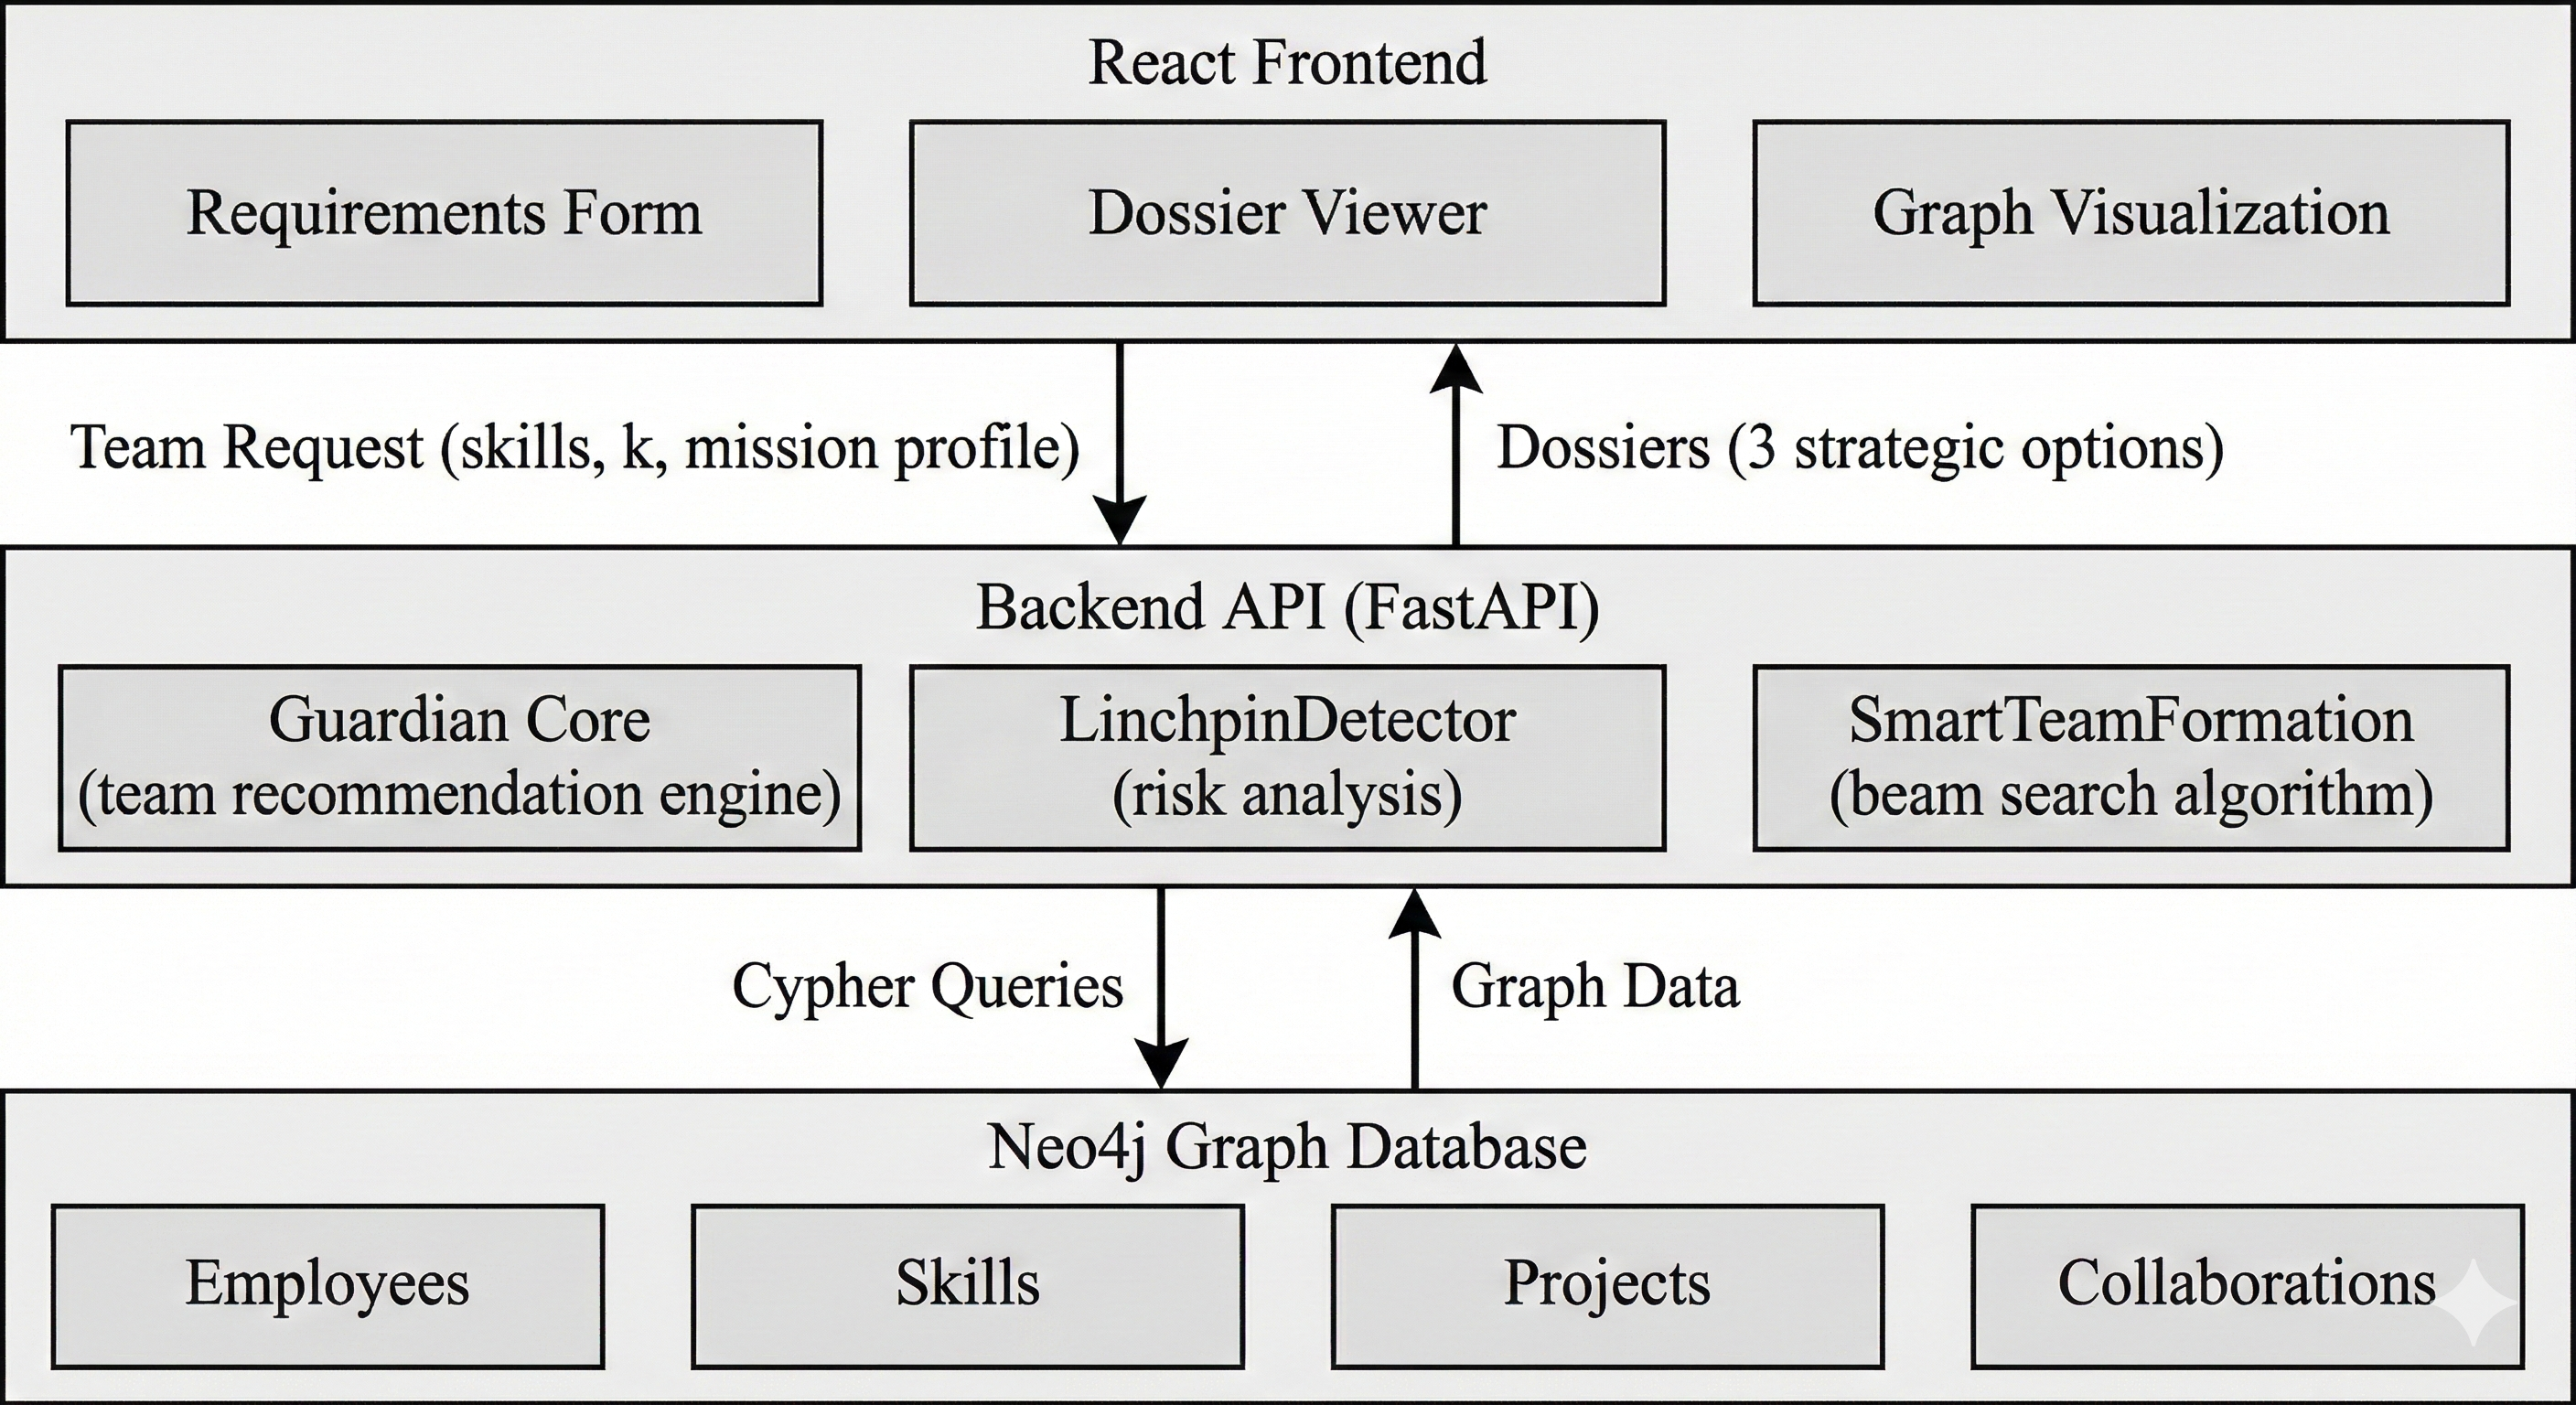
\includegraphics[width=0.48\textwidth]{figuras/fig1_system_architecture.png}
\caption{Arquitectura de tres capas con base de datos de grafos habilitando modelado explícito de colaboración.}
\label{fig:architecture}
\end{figure}

El enfoque basado en grafos habilita razonamiento transparente: los gerentes pueden inspeccionar \textit{por qué} un equipo es riesgoso (ej., "Todos los miembros dependen de Empleado\_027 para experiencia en Docker").

\section{Discusión}

\subsection{Limitaciones}

\textbf{Escala del Dataset:} La validación usó N=150 empleados. Aunque escalable algorítmicamente (NetworkX maneja grafos con $10^4$ nodos), el despliegue en producción a escala empresarial ($>5000$ empleados) requiere algoritmos aproximados de BC \cite{brandes2007variants}.

\textbf{Datos Sintéticos:} Los experimentos emplearon datos generados reflejando distribuciones teóricas. La validación en mundo real con socios industriales es trabajo futuro.

\textbf{Ajuste de Perfiles de Misión:} Las configuraciones de pesos están motivadas teóricamente pero carecen de pruebas A/B extensivas en entornos de producción.

\subsection{Trabajo Futuro}

\textbf{Aprendizaje por Refuerzo:} Las heurísticas actuales son hechas a mano. Agentes de RL (ej., métodos de gradiente de política) podrían aprender funciones de puntuación específicas a misión desde datos de desempeño histórico de equipos.

\textbf{Bandidos Multi-Brazo:} Optimización online de pesos vía bandidos contextuales, adaptándose a dinámicas organizacionales sin reconfiguración manual.

\textbf{Grafos Dinámicos:} Redes de colaboración temporales capturando experiencia y relaciones evolutivas.

\textbf{Analítica Preservando Privacidad:} Minería federada de grafos habilitando análisis de Bus Factor inter-organizacional sin compartir datos.

\subsection{Impacto Práctico}

SmartChimera aborda una brecha crítica: 80\% de gerentes identifican la rotación como el mayor riesgo técnico \cite{robillard2021turnover}, pero carecen de herramientas para mitigación proactiva. Al hacer la optimización de Bus Factor transparente y configurable, nuestro sistema empodera planificación de fuerza laboral basada en evidencia.

\section{Conclusión}

Presentamos SmartChimera, un sistema de ensamblaje de equipos basado en grafos que combina detección híbrida de linchpins con beam search adaptativo. La validación estadística rigurosa (N=500 pruebas) demuestra mejoras significativas sobre baselines estándar de industria: 33\% más alto Bus Factor, 100\% cobertura de habilidades, y 90\% reducción de riesgo (todos p < 0.001).

Las innovaciones clave incluyen: (1) métrica de riesgo híbrida balanceando centralidad de red y carga de trabajo, (2) estrategia de modo dual adaptándose a contexto de misión, y (3) marco de perfiles configurables habilitando optimización guiada por políticas. A diferencia de IA caja negra, SmartChimera provee recomendaciones transparentes y determinísticas adecuadas para entornos regulados.

El trabajo futuro explorará aprendizaje por refuerzo para ajuste automático de pesos y validará el sistema en configuraciones de producción. El fundamento de teoría de grafos ofrece extensibilidad para restricciones adicionales (distribución geográfica, zonas horarias, objetivos de diversidad) sin rediseño fundamental.

Al transformar Bus Factor de métrica pasiva a criterio de optimización accionable, SmartChimera representa un paso hacia organizaciones de software resilientes y basadas en datos.

\section*{Agradecimientos}

Los autores agradecen a la Universidad Nacional de San Agustín por apoyar esta investigación. Reconocemos a la comunidad de código abierto por los frameworks NetworkX, Neo4j y FastAPI que habilitaron este trabajo.

\bibliographystyle{IEEEtran}
\bibliography{referencias_50}

\end{document}
